\section{Proyecto Final de Unidad -  Sistema Recomendacion de Libros} 
\begin{flushleft}

\begin{itemize}
\textbf{1.Antecedentes o Introducción}\\


La palabra Bot proviene de la palabra Robot y es la forma como se le denomina en el lenguaje tecnológico que realiza un procedimiento de manera automática en distintos contextos.
Es un concepto que existe hace casi 50 años, pero con las nuevas herramientas y posibilidades que brinda la época actual, está ganando popularidad dada las diversas aplicaciones que tiene en el mercado.\textbf{ }\\
\textbf{ }\\
\textbf{ }\\
Existen varios tipos de Bots, acá nombraremos algunos de los más conocidos: \textbf{ }\\
\textbf{ }\\
•	Bots de seguimiento en redes sociales (Following Bots)\textbf{ }\\
•	Bots de tráfico para sitios web (Traffic Bots)\textbf{ }\\
•	Bots Informativos\textbf{ }\\
•	Bots de conversación (ChatBots)\textbf{ }\\
\textbf{ }\\
El servicio al cliente en redes sociales está cada día más en tendencia, tenemos claro que es más fácil avisar de la falla en algún servicio en redes sociales que llamar y esperar minutos a ser atendido por una operadora.\textbf{ }\\
\textbf{ }\\
Es biológicamente imposible que un ejecutivo telefónico pueda atender a más de una persona a la vez por lo que las redes sociales y los canales de comunicación de Internet, tales como chat, correo electrónico, o servicios de mensajería móvil son el conducto ideal para atender a más clientes de forma simultánea, ya que un único ejecutivo puede atender 5 o más personas a la vez.\textbf{ }\\
\textbf{ }\\
Si a esta ventaja en atención al cliente le agregaremos bots de primer nivel podemos atender hasta 4 veces más personas que por teléfono con los beneficios adicionales de operar 24/7 todos los días del año.\textbf{ }\\
La idea de tener un bot es complementar la atención humana, haciéndola más eficiente. Apoyar con preguntas frecuentes, consultas simples o tomar datos de manera automática son algunos de los casos más comunes donde se puede aplicar esta tecnología.\textbf{ }\\
\textbf{ }\\
La finalidad de tener una biblioteca con información actualizada y brindar información rápida diferentes medios bibliográficos de la biblioteca, además de poder realizar compras en la pagina web.\textbf{ }\\
El Sistema bibliotecario tiene como objetivo proveer servicios de consulta, pedidos, compras y anulaciones de solicitudes de libros.
\textbf{ }\\
\textbf{ }\\
Para la creación de este sistema para la administración de la información de los distintos libros de la biblioteca, se utilizará la clasificación de los libros así como los diferentes medios que posee la biblioteca como lo son: revistas, libros.
 \textbf{ }\\
\textbf{ }\\
Este sistema será de mucha utilidad para ubicar un libro y otros medios de la biblioteca rápidamente, nos facilitará conocer el status de los libros, la adquisición de nuevos libros y los procesos técnicos por ejemplo catalogación y clasificación de los ejemplares.
\textbf{ }\\
\textbf{ }\\
La finalidad principal de un proyecto de este tipo es la generación, administración y disposición de conocimiento para una comunidad determinada.
Los beneficios académicos es automatizar estos procesos con un sistema de biblioteca que ofrece recomendaciones y compras de libros haciendo la tarea más sencilla para los usuarios.
\textbf{ }\\
\textbf{ }\\
Con la implementación de este sistema se obtendrá la información al instante de los libros, revista, editoriales entre otros. Se podrá obtener una lista de todos los libros en stock, editoriales, etc., y buscar en cualquier momento en base a varios reglas de filtrado. Se podrá organizar la biblioteca por editoriales, autores entre otros.



\textbf{ }\\
\textbf{2.	Titulo}\\
•         Sistema Recomendacion de Libros
\textbf{ }\\
\textbf{ }\\
\textbf{3.	Autores}\\
•	Catari Cabrera, Yofer Nain\textbf{ }\\
•	Acosta Ortiz, Orlando \textbf{ }\\
•	Zegarra Reyes, Roberto\textbf{ }\\
•	Cruz Escalante Richard\textbf{ }\\
•	Mamani Maquera, Jorge Luis\textbf{ }\\
•	Rivas Rios, Marko\textbf{ }\\


\textbf{ }\\

\textbf{4.	Planteamiento del problema}\\
\textbf{4.1. 	Problema}\\

Dificultades en la recepción de clientes para realizar ventas o prestamos de libros y atencion a mensajeria online en redes sociales.\textbf{ }\\
\textbf{ }\\
\textbf{4.2.	Justificación }\\
La propuesta de nuestro proyecto es mejorar la venta o prestamos de libros al cliente por ende incorporaremos un asistente virtual y permitir brindarle recomendaciones de libros similares. 
\textbf{ }\\
\textbf{ }\\
\textbf{4.3.	Alcance }\\
Público en General

\textbf{ }\\
\textbf{ }\\
\textbf{ }\\
\textbf{ }\\
\textbf{ }\\
\textbf{ }\\
\textbf{ }\\
\textbf{ }\\
\textbf{ }\\
\textbf{ }\\
\textbf{5.      Objetivos}\\
\textbf{5.1.   General}\\
-	Poder recomendar diferentes libros a fines al gusto del cliente como podría ser: Autor, Genero, Editorial etc.
\begin{center}
	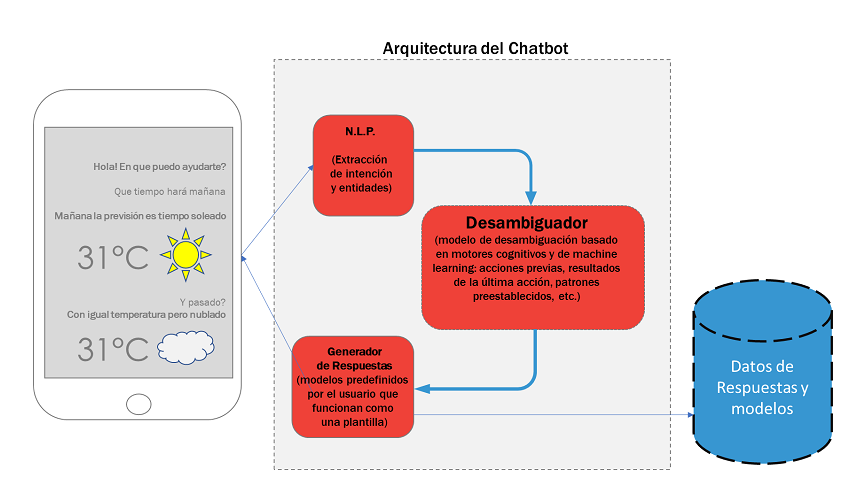
\includegraphics[width=12cm]{./Imagenes/chatbot} 
	\end{center}

\textbf{ }\\

\textbf{5.2.   Específicos}\\

-	Recomendar Libros\\
-	Identificar los gustos literarios del cliente.\\



\textbf{ }\\

\textbf{6.      Referentes teóricos}\\
\textbf{ }\\
En 2019, la facultad de ciencias matematicas y físicas carrera de ingenieria en sistemas computacionales de la Universidad de Guayaquil diseñó y creó un asistente virtual (chatbot) que ha logrado automatizar los procesos manuales de servicios de atención al cliente utilizando Facebook Messenger como canal de comunicación destinados al área comercial. El uso del alojamiento virtual con el diseño de la base de datos logró facilitar el manejo y procesamiento de los datos que son usados por el Asistente Virtual. Mediante el uso de la herramienta de inteligencia artificial Google Dialogflow en el desarrollo del chatbot se logró una mejor comunicación con los clientes, entregando información sobre los productos de línea blanca de forma inmediata. Las opciones de respuestas configuradas en el proceso de interacción entre el cliente y el chatbot son automatizadas basadas en las configuraciones definidas en la I.A. Google Dialogflow, brindado mejoras en el proceso de venta y comunicación con el cliente.\\
\textbf{ }\\
En la tesis Asistente virtual para servicios de la biblioteca de la UCM presentado el 30 de mayo de 2019 por la Facultad de Informática Universidad Complutense de Madrid demostró que el proyecto desarrollado por Mauricio Abbati Loureiro y Jose Luis Moreno Varillas ha consistido en trasladar tecnologías de procesamiento de lenguaje natural para construir un chatbot capaz de resolver consultas relacionadas con el catálogo y la información institucional de las bibliotecas de la Universidad Complutense de Madrid a través de un dispositivo móvil. Para ello, hemos aprovechado las tecnologías de NLP disponibles en el mercado y los dispositivos móviles para ofrecer un sistema con la mayor calidad posible, partiendo de cero con los modelos de entrenamiento para el ámbito de este proyecto. En un principio utilizando la solución ofrecida por IBM con su producto Watson Assistant, con el objetivo de tener un campo de visión mayor en el campo de los chatbot y los NLP. Posteriormente, sustituimos Watson por una solución que fuera de código abierto, para no depender de las limitaciones de utilizar una solución cerrada y con funcionalidades limitadas por el uso de una suscripción gratuita. Esta solución fue spaCy más Rasa. Este conjunto de librerías en Python otorga las herramientas necesarias para la construcción de un NLP y un NLU. Con esto, podemos configurar el sistema de tal forma que tenga la capacidad de dar una respuesta acorde al servicio que se desea ofrecer. Este proyecto ha logrado también, en cierta medida, unificar información, tanto institucional como del catálogo, de las bibliotecas, de manera que el usuario no necesita bucear por las diversas webs de las bibliotecas para obtener información como los números de teléfono, horarios o direcciones. Como conclusión, podemos determinar que el proyecto ha sido desarrollado con éxito, lanzando al público dos aplicaciones para dispositivos iOS y Android, disponibles en sus respectivas tiendas de aplicaciones, así como la implementación del servidor donde se procesan todos los datos enviados por los clientes.\\
\textbf{ }\\

\textbf{7.      Desarrollo de la propuesta}\\

\begin{center}
	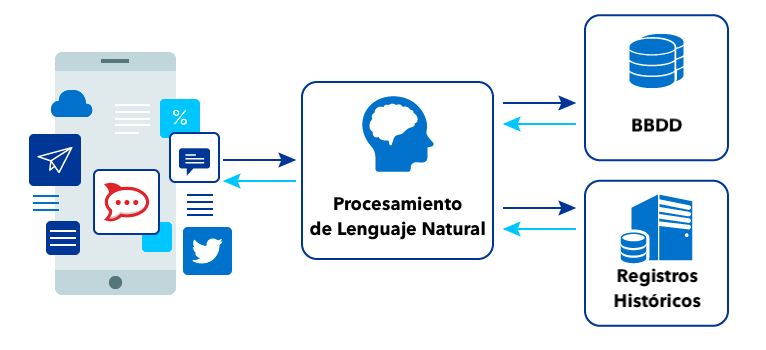
\includegraphics[width=12cm]{./Imagenes/nlp} 
	\end{center}
\textbf{7.1.   Tecnología de información}\\
-	Descripción de productos hardware y software.\\ 
\textbf{ }\\

•	PC core i7 7ta generación, Ram 8GB \\
•	Android \\
•	Visual Code\\
•	MongoDB o MYSQL\\
Funcionalidad de Chatbots( Aquitectura)
\begin{center}
	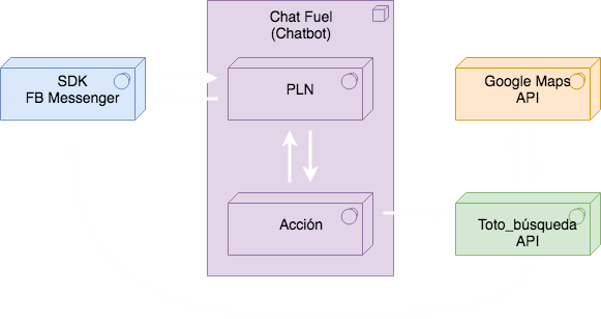
\includegraphics[width=12cm]{./Imagenes/api} 
	\end{center}

\textbf{ }\\
\textbf{7.2.   Metodología, técnicas usadas }\\
-	 desarrollo ágil, la metodología Scrum define perfectamente qué es el método ágil en la gestión de proyectos.

\textbf{7.3.   Metodología, de Desarrollo / Herramientas Usadas}\\
•	 Dialogflow \\
•	 Implementacion de Lenguaje Natural para la Atencion a los Usuarios o Clientes\\
•	 ChatBoot 24/7 \\
•	 Redes Sociales Usados  WhatsApp,Facebook Messenger \\
•	Implementado a un Sitio Web  Biblioteca \\
•	 Base datos Almacenado en Hosting \\

\textbf{ }\\
\textbf{ }\\
\textbf{ }\\
\textbf{ }\\
\textbf{ }\\
\textbf{ }\\
\textbf{ }\\
\textbf{ }\\
\textbf{ }\\
\textbf{ }\\
\textbf{ }\\
\textbf{ }\\
\textbf{ }\\
\textbf{ }\\
\textbf{ }\\
\textbf{ }\\
\textbf{ }\\
\textbf{ }\\
\textbf{ }\\
\textbf{ }\\
\textbf{ }\\
\textbf{ }\\
\textbf{7.4.   Implementacion de Front End y Back End  }\\
-	 Sistema de Biblioteca Implememtado en php,html5,Css3,motor de base datos mysql
-          Nuestro  Portales de Atencion 24 / 7.
\textbf{ }\\
\textbf{ }\\
\textbf{ Front-End}\\
\textbf{ }\\
\textbf{1. Inicio }\\
\begin{center}
	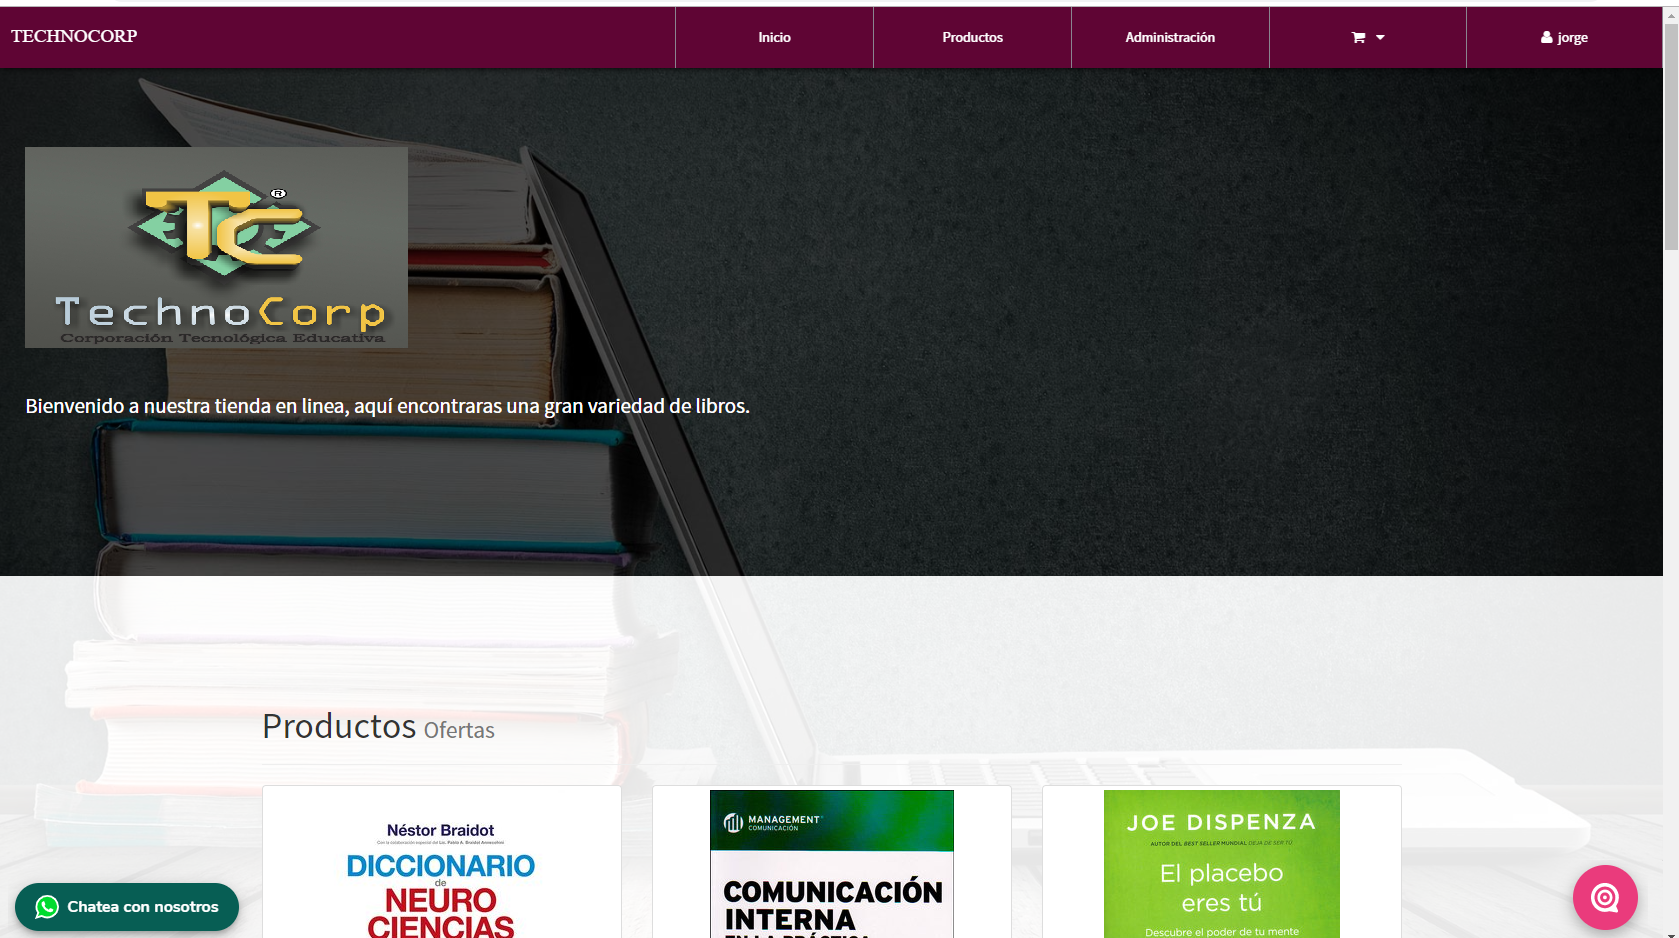
\includegraphics[width=16cm]{./Imagenes/web1} 
\end{center}
\textbf{ }\\
\textbf{2.Chat Bot }\\
\begin{center}
	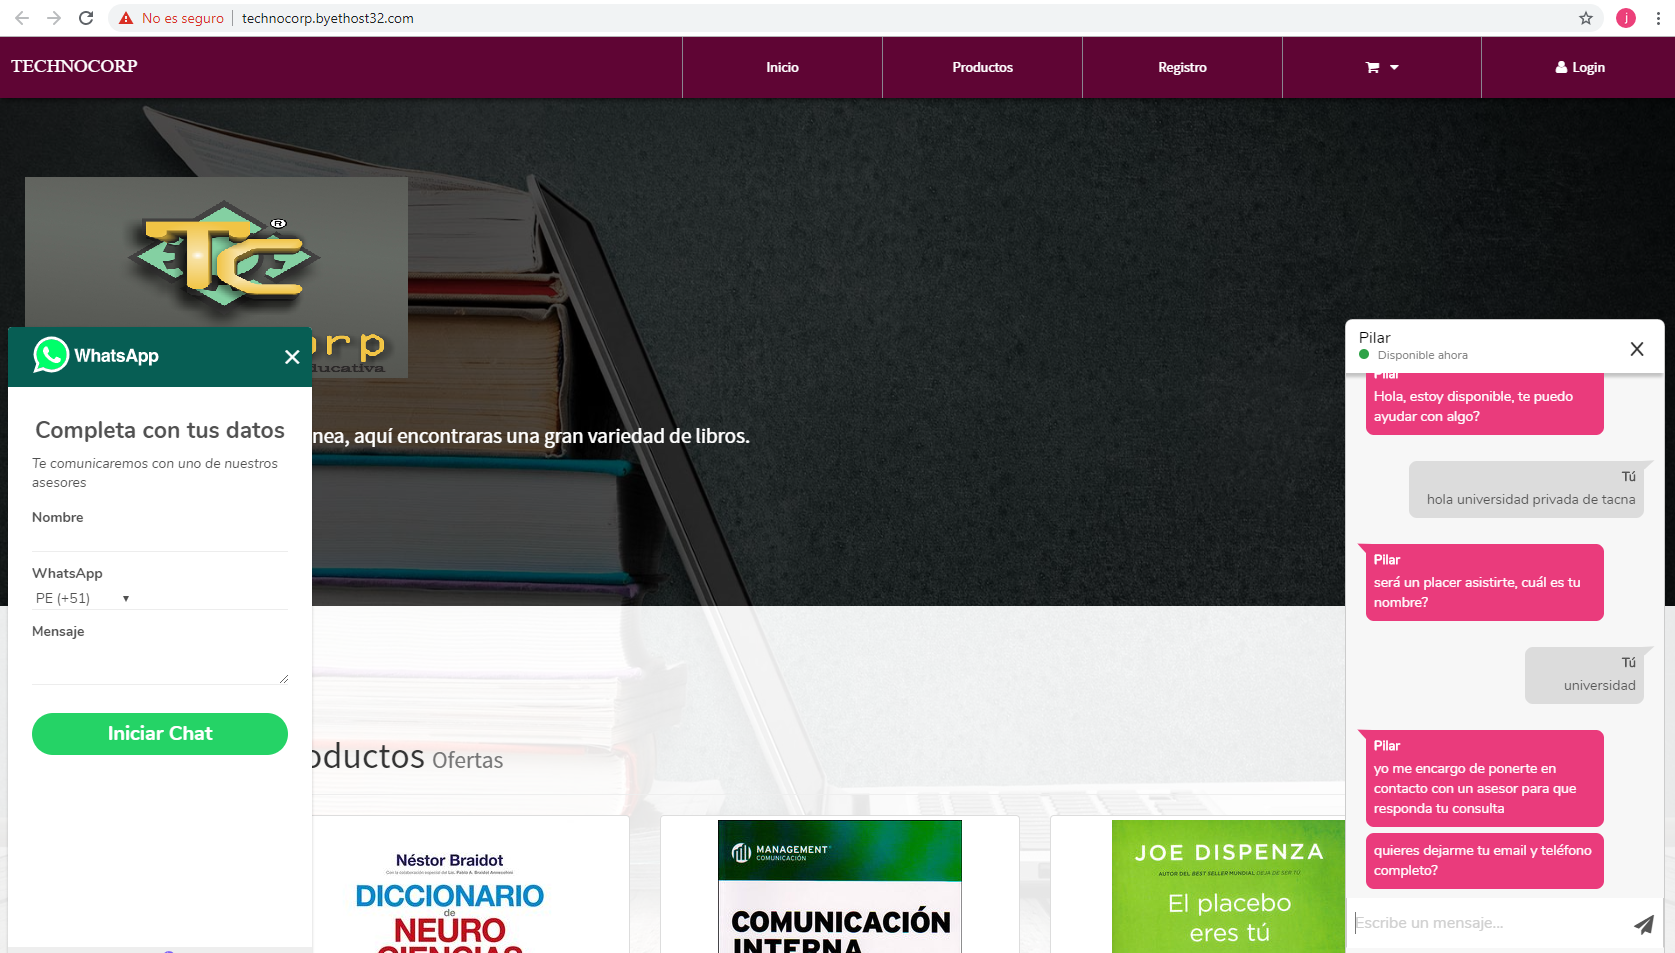
\includegraphics[width=16cm]{./Imagenes/web} 
\end{center}
\textbf{ }\\
\textbf{ }\\
\textbf{3. Productos }\\
\textbf{ }\\
\begin{center}
	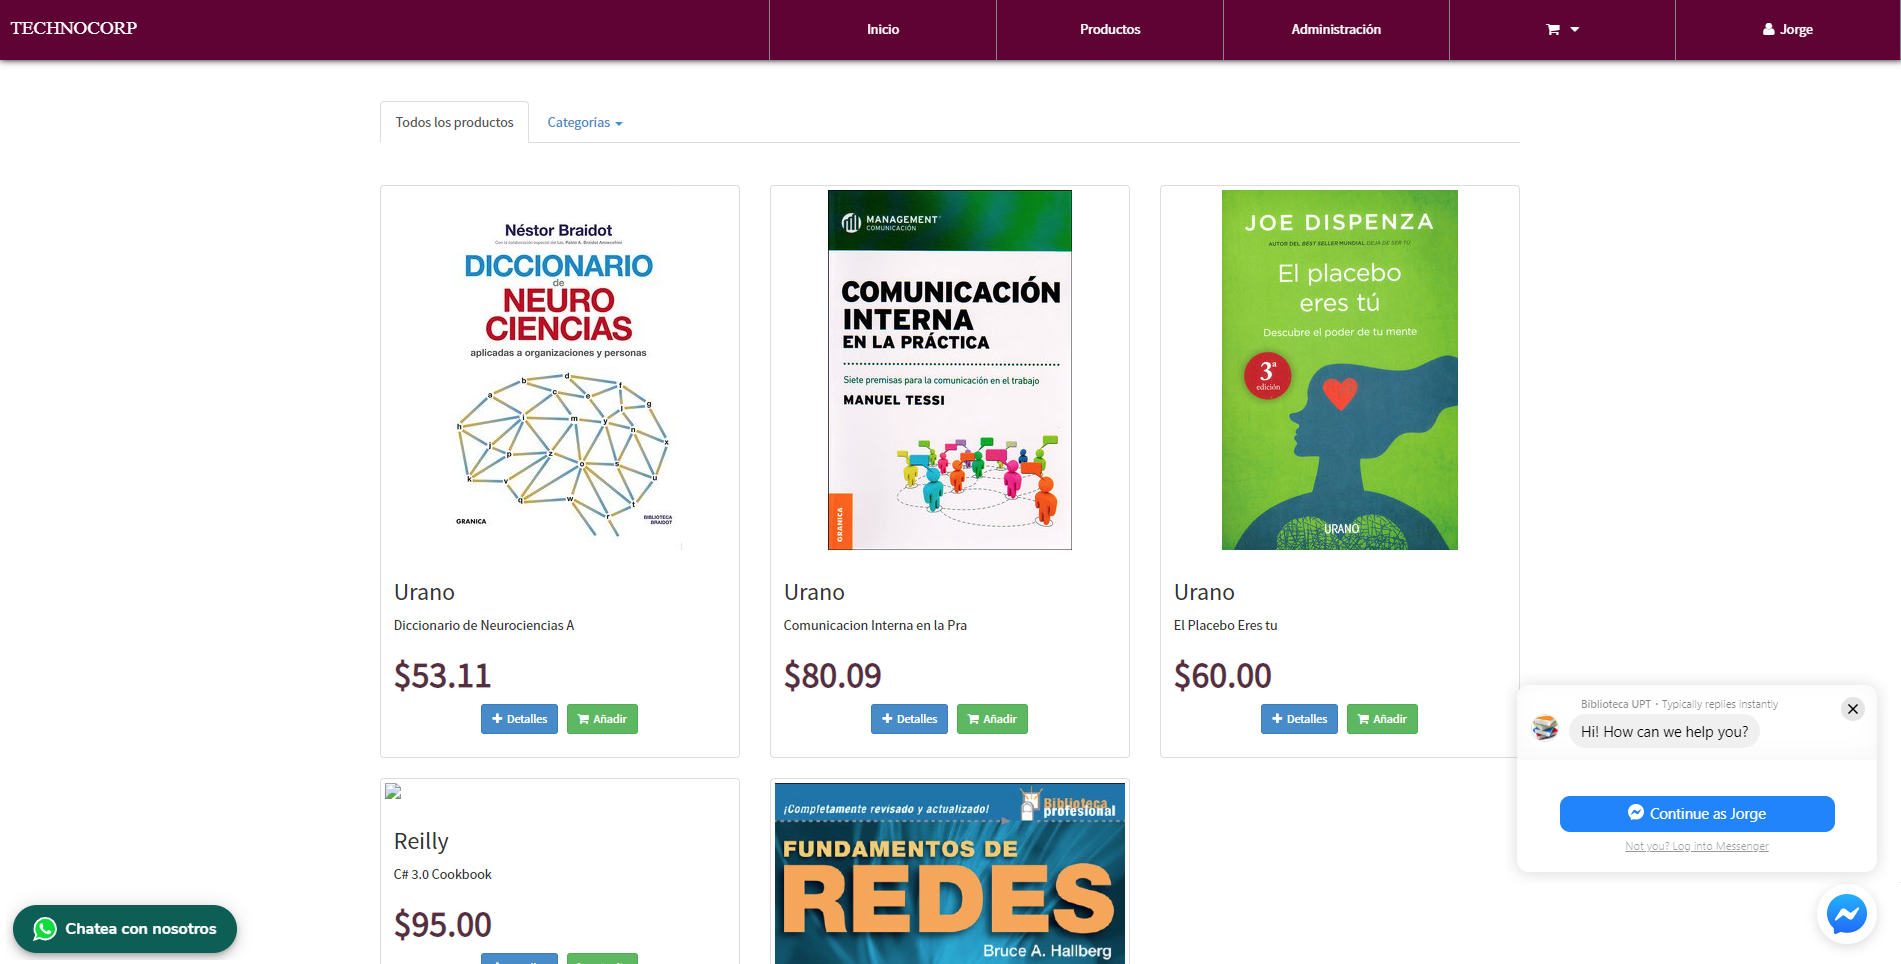
\includegraphics[width=16cm]{./Imagenes/front1} 
\end{center}
\textbf{ }\\
\textbf{ }\\
\textbf{4. Detalle Productos }\\
\textbf{ }\\
\begin{center}
	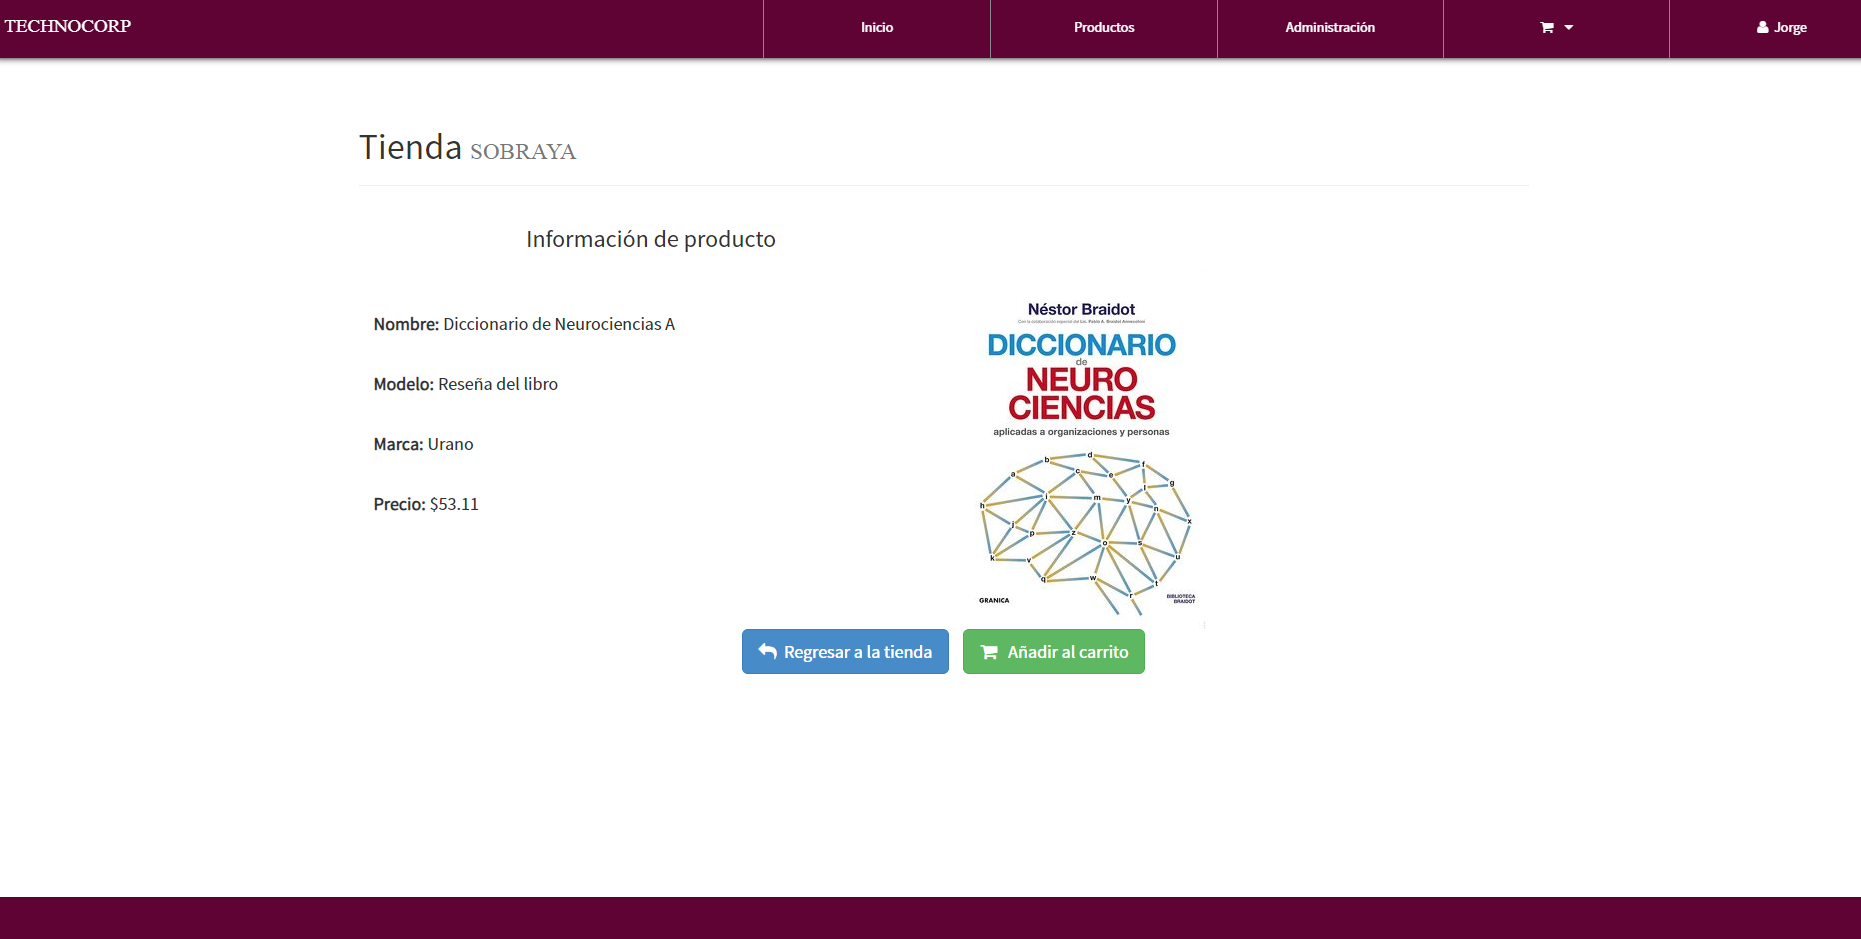
\includegraphics[width=16cm]{./Imagenes/front2} 
\end{center}

\textbf{ }\\
\textbf{ }\\

\textbf{ }\\
\textbf{ }\\

\textbf{ }\\
\textbf{ }\\

\textbf{ }\\
\textbf{ }\\
\textbf{5. Añadir y Confirmar Pedido }\\
\textbf{ }\\
\begin{center}
	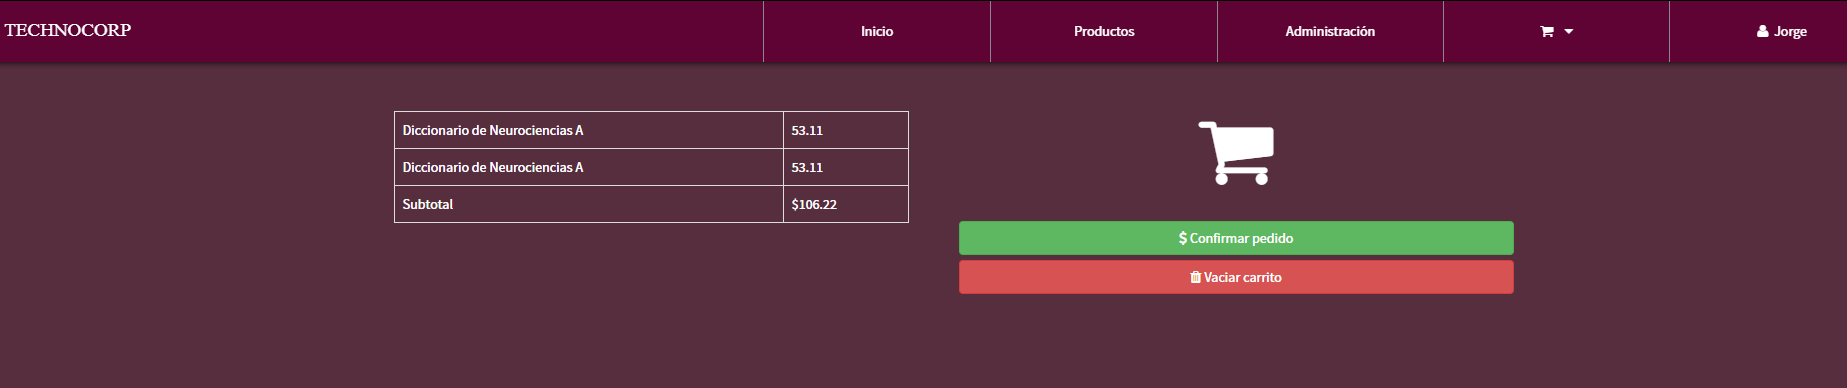
\includegraphics[width=18cm]{./Imagenes/front3} 
\end{center}
\textbf{ }\\
\textbf{ }\\
\textbf{6. Registro de Usuarios }\\
\textbf{ }\\
\begin{center}
	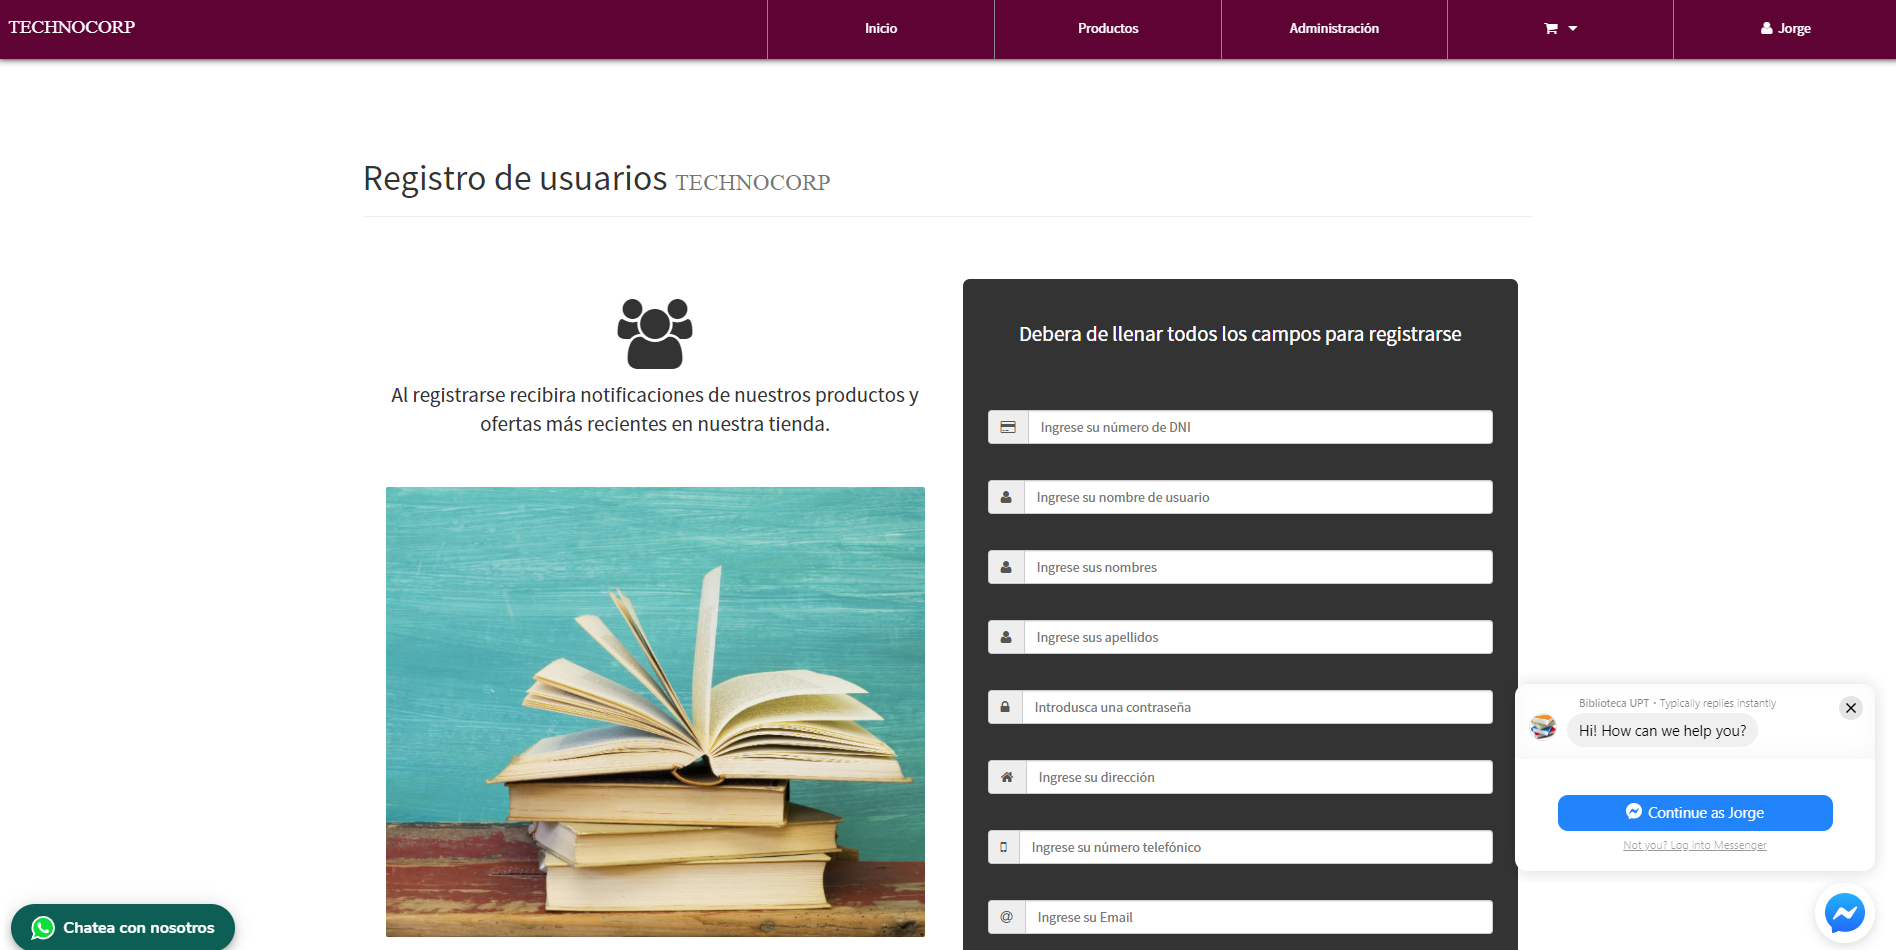
\includegraphics[width=18cm]{./Imagenes/front4} 
\end{center}

\textbf{ }\\
\textbf{ }\\
\textbf{ }\\
\textbf{ }\\
\textbf{ }\\
\textbf{ }\\
\textbf{ }\\
\textbf{ }\\
\textbf{ }\\
\textbf{ }\\
\textbf{ }\\
\textbf{ }\\
\textbf{ }\\
\textbf{ }\\
\textbf{ }\\
\textbf{Back-End}\\
\textbf{ }\\
\textbf{1. Agregar un Nuevo Producto}\\
\textbf{ }\\
\begin{center}
	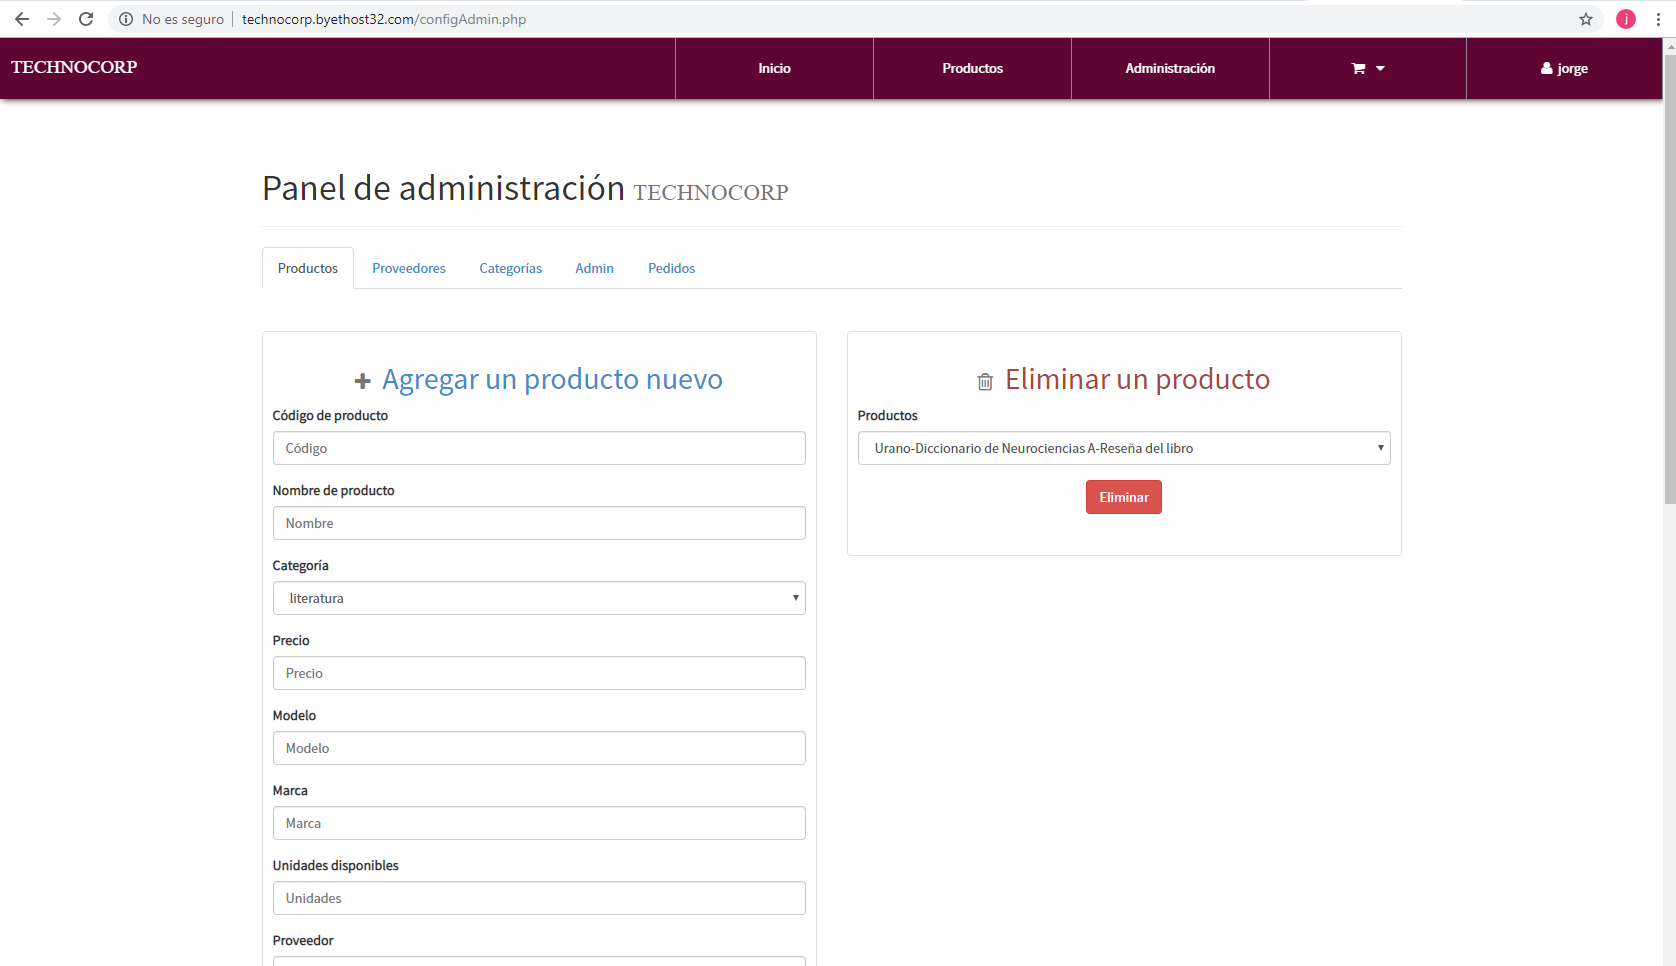
\includegraphics[width=16cm]{./Imagenes/back} 
\end{center}
\textbf{ }\\
\textbf{ }\\
\textbf{2. Agregar un Nuevo Proveedor }\\
\textbf{ }\\
\begin{center}
	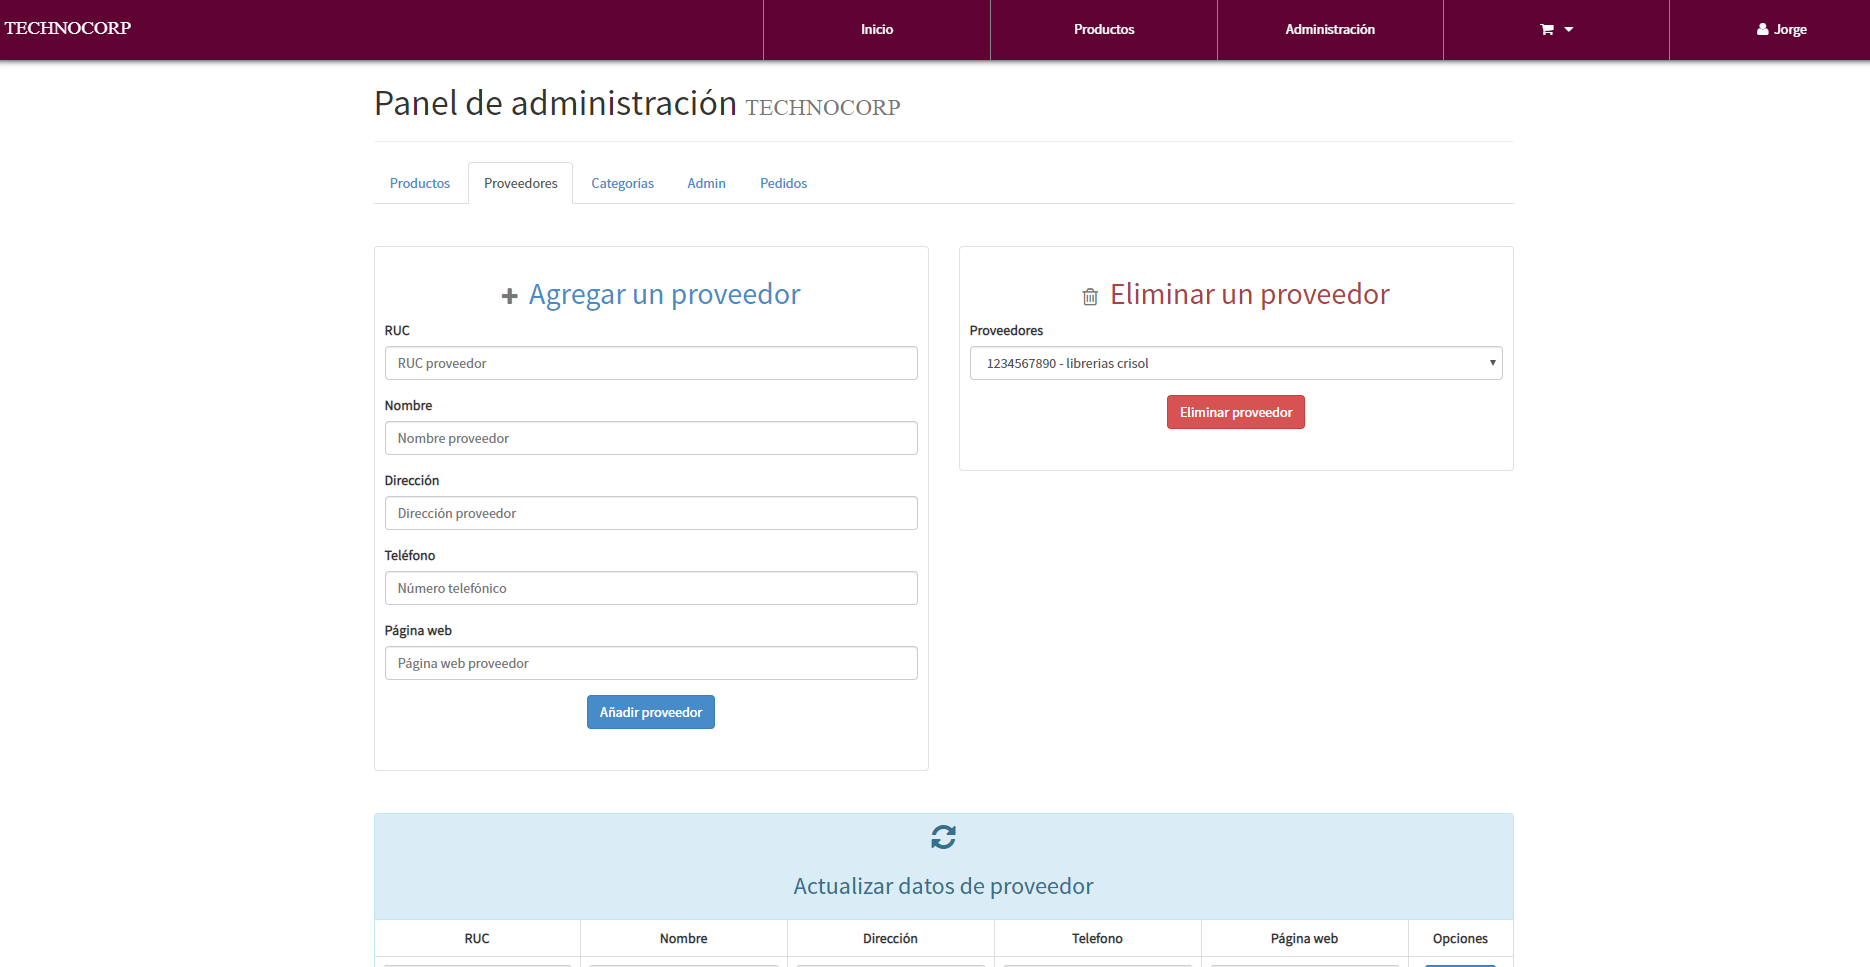
\includegraphics[width=16cm]{./Imagenes/back1} 
\end{center}
\textbf{ }\\
\textbf{ }\\
\textbf{ }\\
\textbf{3. Agregar una Nueva Categoria}\\
\textbf{ }\\
\begin{center}
	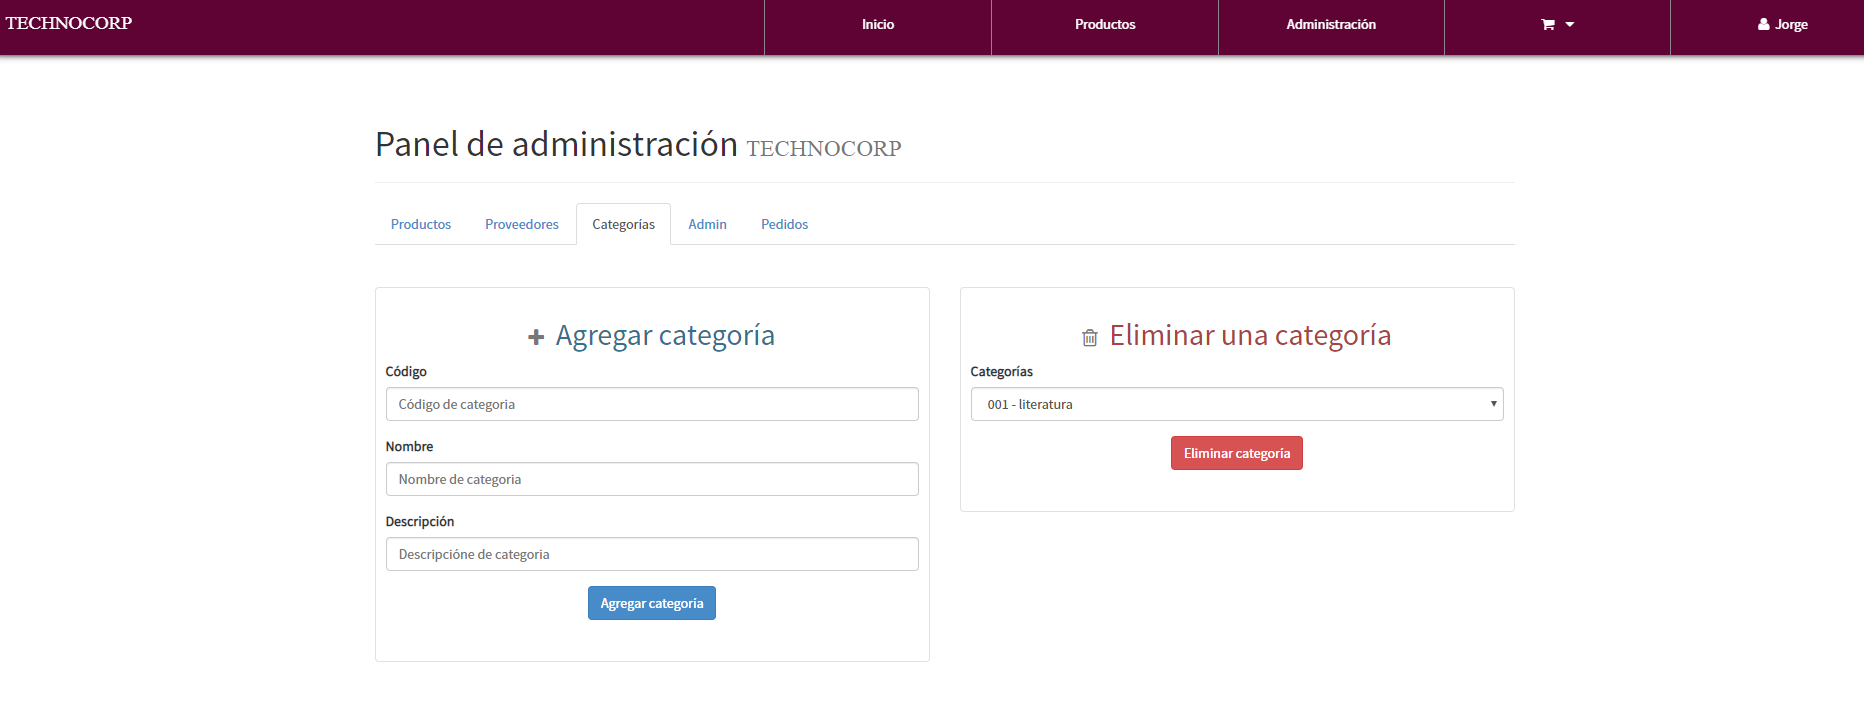
\includegraphics[width=18cm]{./Imagenes/back2} 
\end{center}
\textbf{ }\\
\textbf{ }\\
\textbf{ }\\
\textbf{4. Agregar un Nuevo Adminsitrador}\\
\textbf{ }\\
\begin{center}
	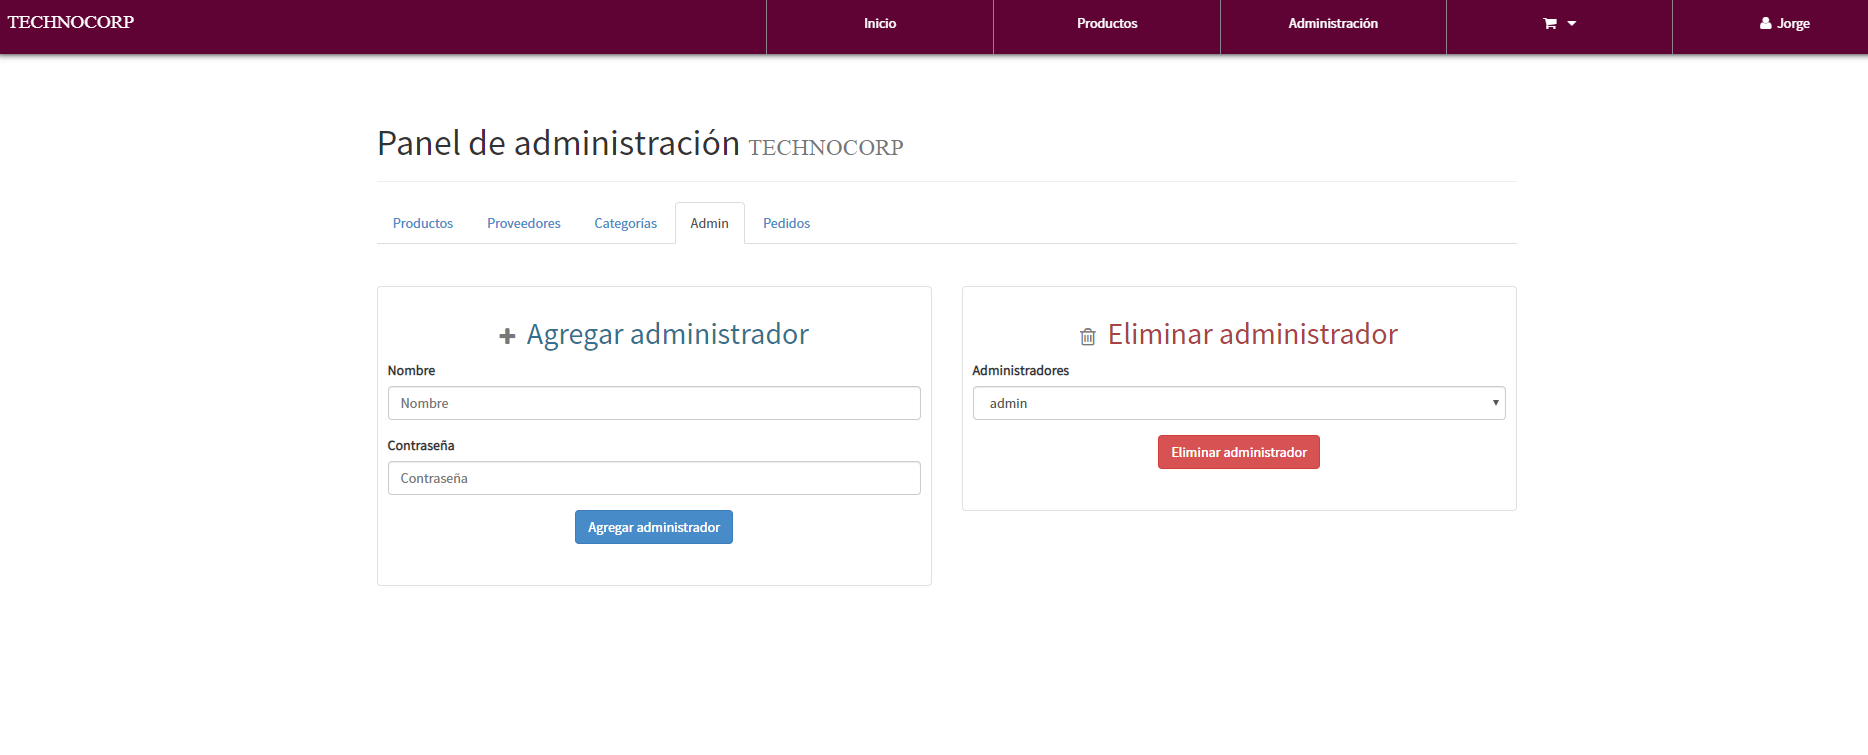
\includegraphics[width=18cm]{./Imagenes/back3} 
\end{center}

\textbf{ }\\
\textbf{ }\\
\textbf{ }\\
\textbf{ }\\
\textbf{ }\\
\textbf{ }\\
\textbf{ }\\
\textbf{ }\\
\textbf{ }\\
\textbf{ }\\
\textbf{ }\\
\textbf{5. Eliminar Pedidos}\\
\textbf{ }\\
\begin{center}
	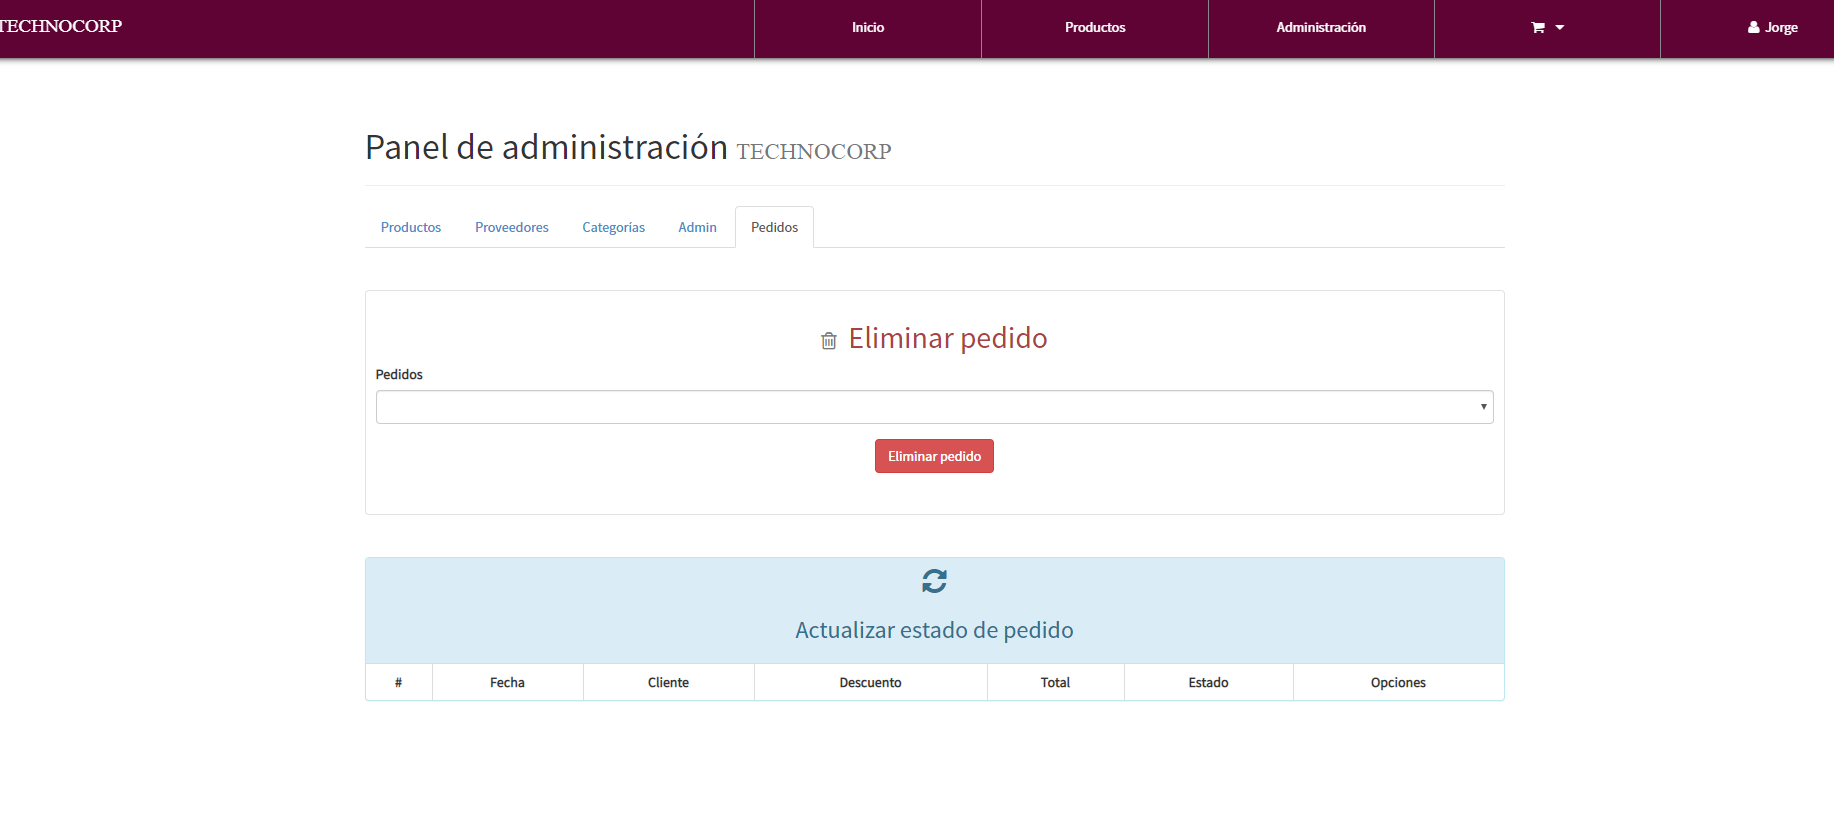
\includegraphics[width=18cm]{./Imagenes/back4} 
\end{center}
\textbf{ }\\
\textbf{ }\\


\textbf{ }\\
\textbf{8.      Cronograma (personas, tiempo, otros recursos) }\\
\textbf{ }\\

\textbf{ }\\
\begin{center}
	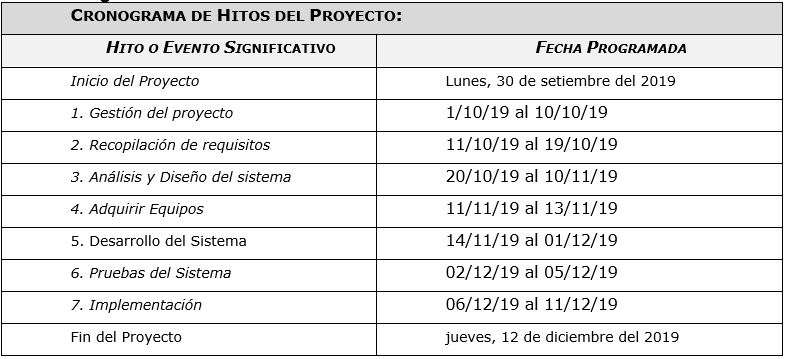
\includegraphics[width=12cm]{./Imagenes/cronograma} 
	\end{center}
\textbf{ }\\
\textbf{ }\\
\textbf{ }\\

\textbf{ }\\
Link de Proyecto Biblioteca
http://technocorp.byethost32.com/index.php

\textbf{8.  Conclusiones y Recomendaciones (comentar dificultades y retos en el desarrollo del trabajo)}\\
\textbf{ }\\
-	En la actualidad es necesario contar con este tipo de tecnología ya que mejora  experiencia del usuario por otro lado también nos lleva a recurrir a múltiples tecnologías.\textbf{ }\\
-	Hoy en día el uso de los asistentes virtuales es una herramienta muy importante de interacción porque gracias a ella existe una nueva forma de interactuar con los demás. De esta manera se hace patente la relación entre la tecnología y las personas.\textbf{ }\\
\textbf{ }\\
\textbf{ }\\
\textbf{9. Bibliografia}\\

- https://medium.com/parkode/los-chatbots-en-la-actualidad-1d0aa68447ce\\
- https://www.diariolibre.com/estilos/buena-vida/bienvenidos-a-la-era-de-los-chatbots- NY7616609\\
- https://medium.com/@cogniapps/historia-de-los-chatbots-bd71f3fd914a\\
- https://www.xataka.com/historia-tecnologica/asi-era-eliza-el-primer-bot- conversacional-de-la-historia\\
- https://es.wikipedia.org/wiki/Mensajer\%C3\%ADa\_instant\%C3\%A1nea\\
- https://planetachatbot.com/chatbots-revolucion-e-innovacion-en-empresas- f0fcb4e98916\\
- http://repositorio.ug.edu.ec/bitstream/redug/45108/1/B-CISC-PTG-1665\%20Mart\%c3\%adnez\%20Carpio\%20Juan\%20Andr\%c3\%a9s.pdf\\


\end{itemize} 


\end{flushleft}